\section{Конструкторский раздел}

\subsection{IDEF0 диаграмма}

На рисунках \ref{fig:a0} -- \ref{fig:a1} ниже приведена IDEF0 диаграмма разрабатываемого загружаемого модуля ядра.

\begin{figure}[H]
	\centering
	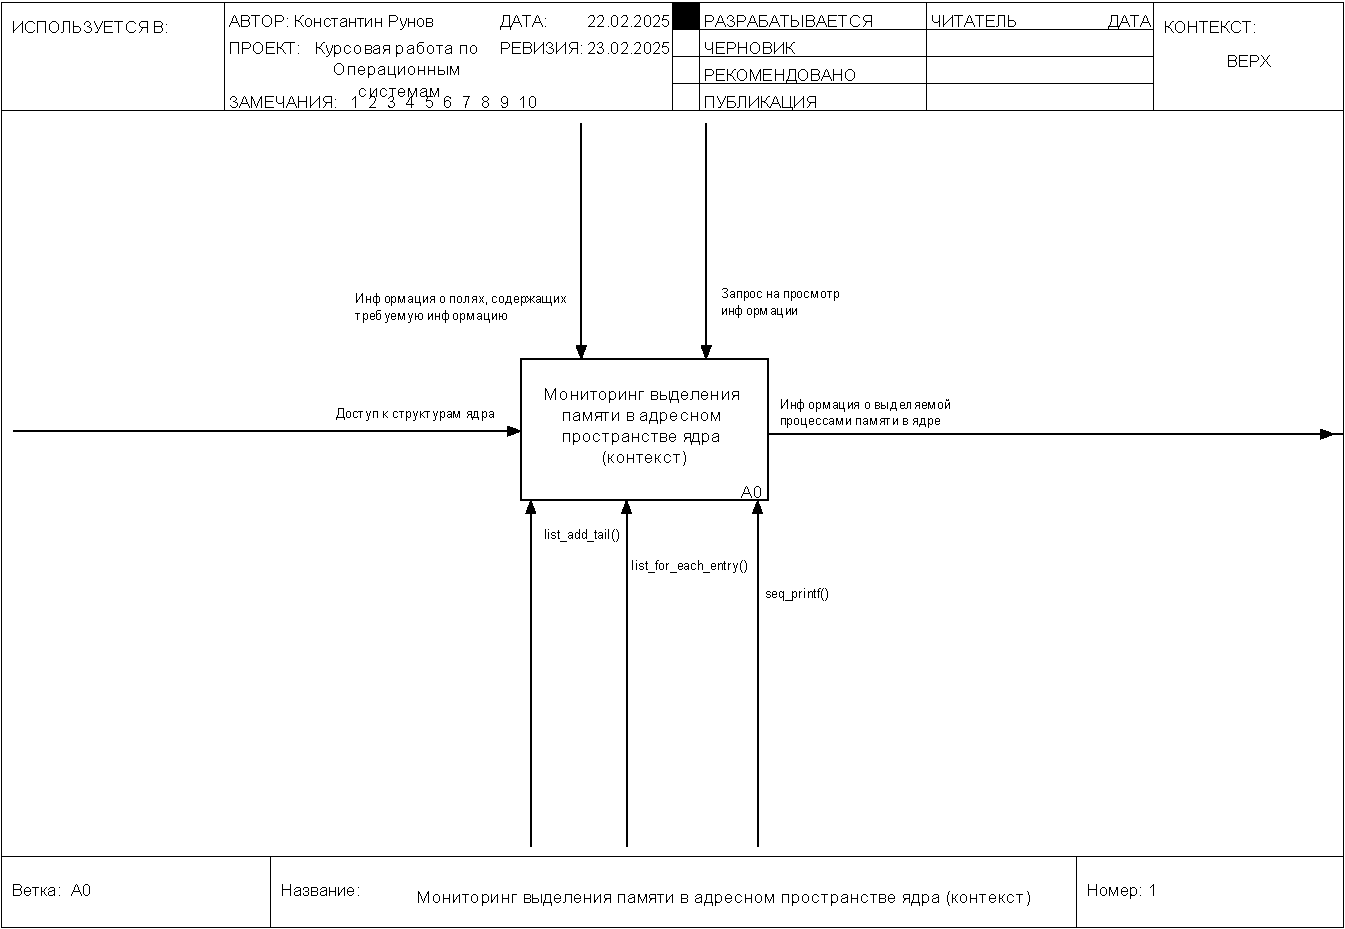
\includegraphics[width=\textwidth]{diag/idef0-A0.pdf}
	\caption{Диаграмма уровня A0}
	\label{fig:a0}
\end{figure}

\begin{figure}[H]
	\centering
	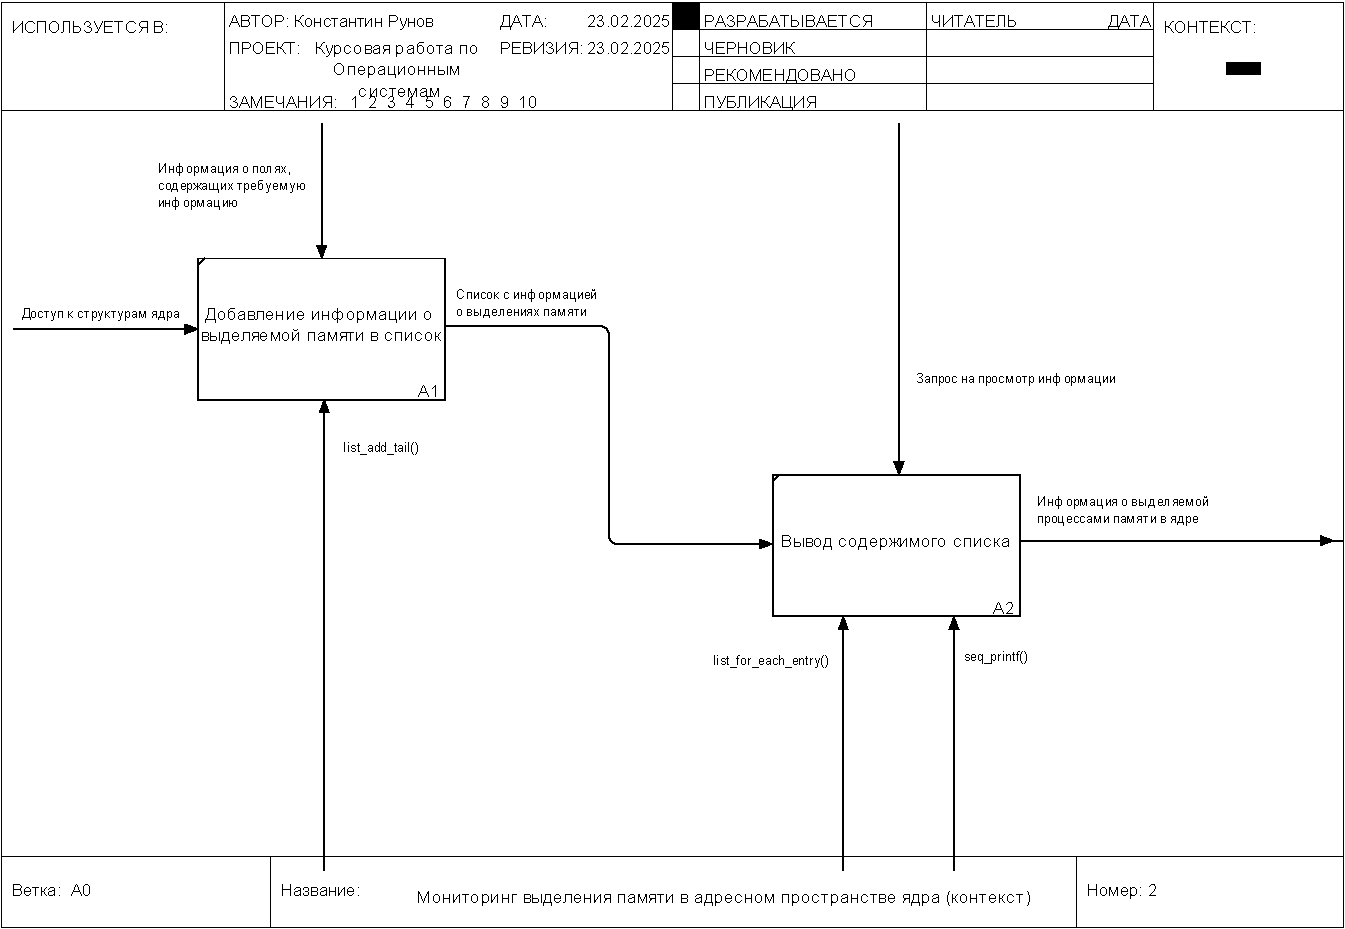
\includegraphics[width=\textwidth]{diag/idef0-A1.pdf}
	\caption{Диаграмма уровня A1}
	\label{fig:a1}
\end{figure}

\newpage

\subsection{Схемы алгоритмов}

На рисунках \ref{fig:kmalloc} -- \ref{fig:show} ниже приведены схемы алгоритмов разрабатываемого загружаемого модуля ядра.

\begin{figure}[H]
	\centering
	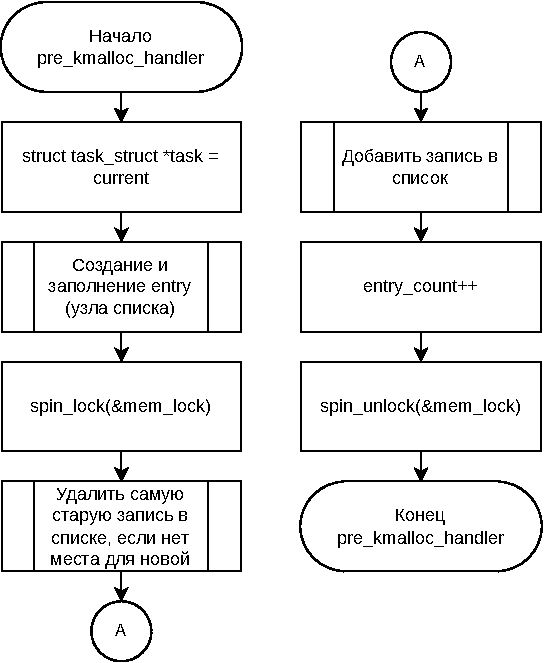
\includegraphics[width=0.7\textwidth]{diag/kmalloc.pdf}
	\caption{Схема pre\_kmalloc\_handler}
	\label{fig:kmalloc}
\end{figure}

\begin{figure}[H]
	\centering
	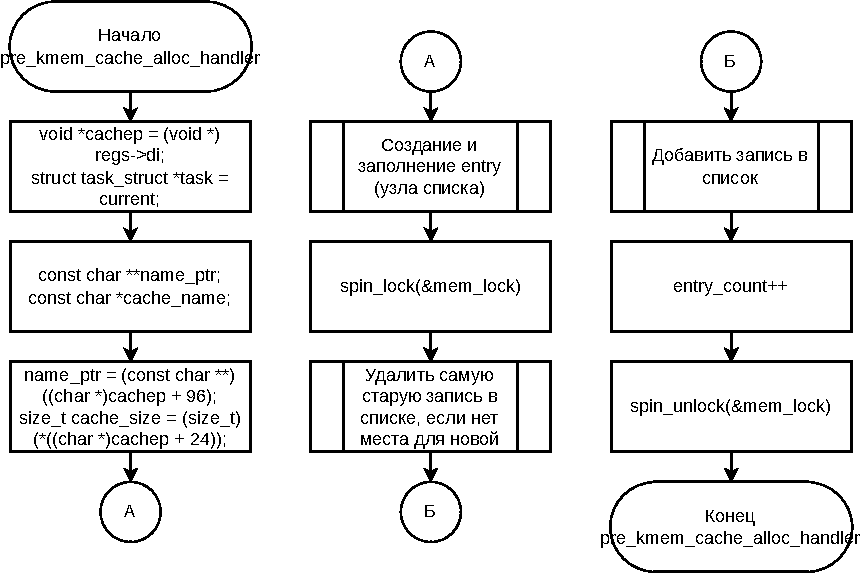
\includegraphics[width=\textwidth]{diag/kmem-cache.pdf}
	\caption{Схема pre\_kmem\_cache\_alloc\_handler}
	\label{fig:kmem}
\end{figure}

\begin{figure}[H]
	\centering
	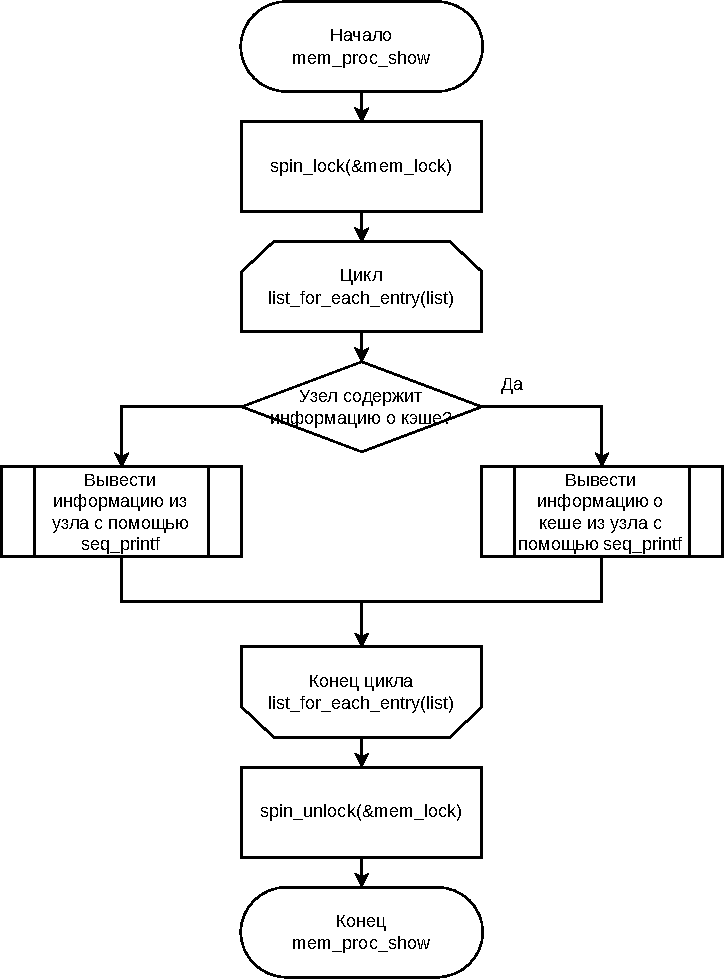
\includegraphics[width=0.9\textwidth]{diag/proc-show.pdf}
	\caption{Схема mem\_proc\_show}
	\label{fig:show}
\end{figure}

%1. IDEF0 A0 или A1
%2. Схемы алгоритмов по ГОСТу
%3. Структуры ядра можно

%В данном разделе будет приведен алгоритм работы реализуемого статического сервера, использующего модуль prefork для мультипроцессной обработки, а также системный вызов select для реализации мультиплексирования.
%
%\subsection{Алгоритм работы сервера}
%
%На рисунках \ref{fig:main} -- \ref{fig:hc} ниже представлены схемы алгоритмов, используемых в процессе работы статического сервера.
%
%\begin{figure}[H]
%	\centering
%	\includegraphics[scale=1]{diag/main.pdf}
%	\caption{Схема алгоритма работы main}
%	\label{fig:main}
%\end{figure}
%
%\begin{figure}[H]
%	\centering
%	\includegraphics[scale=1]{diag/spawn\_workers.pdf}
%	\caption{Схема алгоритма работы spawn\_workers}
%	\label{fig:sw}
%\end{figure}
%
%\begin{figure}[H]
%	\centering
%	\includegraphics[scale=1]{diag/handle\_client.pdf}
%	\caption{Схема алгоритма работы handle\_client}
%    \label{fig:hc}
%\end{figure}
%
%\subsection*{Вывод}
%
%В данном разделе был приведен алгоритм работы реализуемого статического сервера, использующего модуль prefork для мультипроцессной обработки, а также системный вызов select для реализации мультиплексирования.
